%==============================================================================
% Radar Pulse Classification under Low SNR: A Controlled Comparison of
% Time-Frequency Representations and Deep Architectures
%
% Target: IEEE journal (IEEEtran, journal mode). Compile: see paper/README.md.
%
% Conventions used in this draft:
%   \TODO{...}  -- something the authors must supply/verify (esp. citations).
%   \PENDING{...} -- a number that fills in once the multi-seed runs finish.
%==============================================================================
\documentclass[journal]{IEEEtran}

\usepackage{graphicx}
\usepackage{amsmath,amssymb}
\usepackage{booktabs}
\usepackage{array}
\usepackage{url}
\usepackage[hidelinks]{hyperref}
\usepackage{orcidlink}
\usepackage{xcolor}

% Find figures in the analysis/ and results/ trees without copying them.
\graphicspath{{../analysis/}{../experiments/results/}{figures/}}

% Draft helpers -- remove (or redefine to {}) before submission.
\newcommand{\TODO}[1]{\textcolor{red}{[\textbf{TODO:} #1]}}
\newcommand{\PENDING}[1]{\textcolor{blue}{[\emph{pending: #1}]}}

\begin{document}

\title{Robustness of Time--Frequency Representations for Radar Pulse
Classification under Low Signal-to-Noise Ratio}

\author{Kaan~Emre~Evci~\orcidlink{0009-0001-4521-9327}% <-this % stops a space
\thanks{K.~E. Evci is an independent researcher, Istanbul, T\"urkiye
(e-mail: kemree926@gmail.com; ORCID: 0009-0001-4521-9327).}
\thanks{This work was carried out independently, without institutional funding or
support.}
\thanks{Code and data-generation pipeline:
\url{https://github.com/Adrift21/radar-pulse-classification}.}}

\markboth{Preprint --- Manuscript in preparation}%
{Evci: Robustness of Time--Frequency Representations for Radar Pulse Classification}

\maketitle

%------------------------------------------------------------------------------
\begin{abstract}
Automatic classification of radar pulse waveforms is a core task in electronic
support and electronic warfare, where signals are typically observed at low
signal-to-noise ratio (SNR). Most reported systems are evaluated near clean
conditions, leaving open how the choice of time--frequency (TF) representation
governs behaviour as SNR degrades. We present a controlled study that isolates
this factor: eight radar waveform families (LFM, NLFM, Barker, Frank, polyphase
P1--P4, Costas, CW, and stepped/frequency-hopping) are classified from three TF
representations---the short-time Fourier transform (STFT), the Choi--Williams
distribution (CWD), and the Wigner--Ville distribution (WVD)---using three
architectures (a compact custom CNN, ResNet-50, and ViT-Small) on a single,
frozen train/validation/test split spanning $-10$ to $+20$~dB. Across 40{,}000
synthetic signals we find that the choice of representation dominates: STFT and
CWD reach $\approx$98\% and 97\% overall accuracy respectively, while the raw WVD
collapses to $\approx$89\%. The gap is entirely concentrated at low SNR---at
$-10$~dB the WVD falls to $24.8\%$ (near the 8-class chance level) versus
$\approx$85\% for STFT/CWD, a 60-point difference that vanishes above $+2$~dB. We
attribute this to noise-driven cross-term interference in the quadratic WVD, and
support the interpretation with a qualitative TF analysis and a per-SNR confusion
breakdown. Architecture is a secondary factor: the 1.77M-parameter custom CNN
matches or exceeds ResNet-50 and ViT-Small at $\sim$13$\times$ fewer parameters.
\end{abstract}

\begin{IEEEkeywords}
Radar pulse classification, time--frequency analysis, Wigner--Ville distribution,
Choi--Williams distribution, deep learning, SNR robustness, electronic warfare.
\end{IEEEkeywords}

%==============================================================================
\section{Introduction}
%==============================================================================
\IEEEPARstart{I}{ntra}-pulse modulation recognition is a core function of
electronic support measures (ESM) and electronic intelligence: an intercepting
receiver must label each incoming pulse by its modulation family, frequently from
a single observation and without cooperation from the emitter. The task is made
harder by modern low-probability-of-intercept (LPI) radars, which deliberately
spread their energy in time and frequency using waveforms such as linear and
non-linear frequency modulation, Barker and polyphase (Frank, P1--P4) codes,
Costas and stepped frequency hopping, and continuous wave~\cite{pace2009lpi}. By
design, such emitters are observed at low signal-to-noise ratio (SNR), so a
practically useful classifier must remain reliable precisely where the signal is
weakest.

A now-standard approach recasts this signal problem as image recognition: the
intercepted pulse is mapped to a two-dimensional time--frequency (TF)
representation and classified with a convolutional or, more recently, a
transformer network~\cite{zhang2017cnn,kong2018cnn,qu2018intrapulse}. The TF
representation is the crux of this pipeline, because it determines what structure
is exposed to the network. Yet the representations in common use embody very
different trade-offs. The short-time Fourier transform (STFT) is linear and
artefact-free but resolution-limited by its window. Quadratic (Cohen's-class)
distributions such as the Wigner--Ville distribution (WVD) achieve far higher
time--frequency resolution, at the cost of cross-terms; reduced-interference
distributions such as the Choi--Williams distribution (CWD) introduce a kernel
that suppresses those cross-terms~\cite{choi1989,cohen1989,jeong1992kernel}.
These trade-offs interact with noise in ways that should matter most at low SNR,
yet two aspects remain under-examined in the radar-classification literature.
First, the TF representation is typically fixed a priori rather than compared
under identical conditions. Second, accuracy is often reported at a single,
favourable SNR, leaving the low-SNR behaviour---the operationally decisive
regime---uncharacterised. Section~\ref{sec:related} details how prior work
relates to these two gaps.

This paper isolates the effect of the TF representation through a controlled
comparison. We hold the dataset, the frozen split, and the training protocol
fixed, and vary only (i) the representation---STFT, CWD, or WVD---and (ii) the
architecture---a compact custom CNN, ResNet-50, or ViT-Small. Every model is
trained and evaluated across the full $-10$ to $+20$~dB range on 40{,}000
synthetic signals, and accuracy is reported \emph{as a function of SNR} rather
than at a single operating point. This design lets us attribute performance
differences to the representation and the architecture separately, and to
characterise how each degrades as SNR falls.

Our central finding is that the representation, not the architecture, dominates:
STFT and CWD are robust across the SNR range, whereas the raw WVD collapses at low
SNR---by 60 accuracy points at $-10$~dB---because noise-induced cross-terms fill
the TF plane and bury the signature. Above $+2$~dB the three representations are
essentially indistinguishable, which is precisely why single-operating-point
evaluations miss the effect.

\noindent\textbf{Contributions.}
\begin{itemize}
\item A controlled 3$\times$3 comparison (representation $\times$ architecture) of
radar pulse classification on a shared, frozen SNR-stratified split, with
per-SNR and per-class analysis.
\item Evidence that the representation, not the architecture, is the dominant
factor, and that the raw WVD collapses at low SNR while STFT and CWD remain
robust---a 60-point accuracy gap at $-10$~dB.
\item A mechanistic account of the collapse in terms of noise-driven cross-term
interference, supported by qualitative TF imagery and a per-SNR confusion
analysis.
\item A resource-efficiency finding: a 1.77M-parameter CNN matches ImageNet-scale
backbones on this task, at an order of magnitude fewer parameters.
\end{itemize}

%==============================================================================
\section{Related Work}
\label{sec:related}
%==============================================================================
\textbf{Intra-pulse modulation recognition.} Recognising the intra-pulse
modulation of intercepted radar pulses is a long-standing problem in electronic
support, driven by the proliferation of low-probability-of-intercept (LPI)
waveforms---frequency-modulated, phase-coded, and frequency-hopping
families---whose design and detection are treated comprehensively
by~\cite{pace2009lpi}. Classical recognisers relied on hand-crafted features
(instantaneous frequency, phase statistics, and transform-domain descriptors)
followed by a statistical classifier. More recent work reframes the task as image
recognition over a time--frequency (TF) image and applies deep networks:
convolutional models have been trained on TF images for LPI radar waveform
recognition~\cite{kong2018cnn,huynhthe2021cwdtfa,huynhthe2021danet}, for radar
intra-pulse modulation recognition~\cite{qu2018intrapulse}, and with adaptive
feature construction and attention mechanisms~\cite{huang2023lpi}; the same
TF-plus-CNN methodology extends to the closely related recognition of
communications (cognitive-radio) waveforms drawn from overlapping
families~\cite{zhang2017cnn}. These systems report strong accuracy, but two
limitations recur and motivate our study: the TF representation is chosen a priori
rather than compared, and results are frequently summarised at a single,
favourable SNR.

\textbf{Time--frequency representations.} The choice of TF representation governs
what structure the classifier sees, and the available representations embody very
different trade-offs~\cite{boashash2016}. The linear STFT/spectrogram is
artefact-free but resolution-limited by its window. Cohen's class of bilinear
distributions~\cite{cohen1989} trades this off differently: the Wigner--Ville
distribution attains the highest joint resolution but generates cross-terms, and
reduced-interference distributions temper them through a smoothing kernel---the
Choi--Williams exponential kernel~\cite{choi1989} being the canonical instance,
later generalised by systematic kernel-design procedures~\cite{jeong1992kernel}.
Tellingly, radar-recognition systems tend to commit to a single such
representation---the WVD in~\cite{huynhthe2021danet} or the CWD
in~\cite{huynhthe2021cwdtfa}, for example---and awareness that cross-terms interact
poorly with noise has prompted work on kernels with stronger anti-noise behaviour
than the raw CWD~\cite{qu2018intrapulse}. What remains missing, and what we
provide, is a \emph{controlled} comparison of STFT, CWD, and WVD under identical
data, split, and training, with accuracy resolved as a function of SNR so that the
low-SNR regime is characterised explicitly rather than averaged away.

\textbf{Deep architectures.} On the modelling side, two families dominate TF-image
classification: deep convolutional networks such as ResNet~\cite{he2016resnet} and,
more recently, vision transformers~\cite{dosovitskiy2021vit}, both commonly
initialised from ImageNet weights via transfer learning and readily available
through model libraries~\cite{wightman2019timm}. Prior radar studies tend to adopt
a single backbone---often a bespoke CNN~\cite{kong2018cnn,qu2018intrapulse} or a
pretrained network---without an apples-to-apples comparison at matched capacity.
We instead benchmark a compact custom CNN against a pretrained ResNet-50 and a
capacity-matched ViT-Small under a single protocol, which lets us separate the
effect of architecture from that of the representation and quantify how little
architectural complexity this task actually requires.

%==============================================================================
\section{Dataset and Signal Model}
%==============================================================================
The dataset comprises 40{,}000 synthetic complex-baseband signals, 5{,}000 per
class for eight classes, generated in MATLAB. Each signal is 2{,}048 samples long
at a $100$~MHz sample rate ($20.48~\mu$s), with pulse width drawn uniformly from
$[1,20]~\mu$s (Frank and polyphase use $[4,20]~\mu$s so their $N^2$ chips remain
oversampled) and randomised zero-padding position. Table~\ref{tab:classes}
summarises the classes.

Each signal is assigned a target SNR from a 16-point grid spanning $-10$ to
$+20$~dB in $2$~dB steps. Crucially, additive white Gaussian noise (AWGN) is
\emph{not} stored: it is applied at training time (Section~\ref{sec:method}),
measured against the active-region (pulse) power rather than the padded frame, so
a clean signal can be paired with different noise realisations across epochs.
Generation is fully seeded (per-sample seed $= 42 + \text{index}$) for
reproducibility.

Within each class, parameters are randomised to prevent the network from latching
onto a single template (Table~\ref{tab:classes}). LFM sweeps a bandwidth
$B\in[5,20]$~MHz in either direction; NLFM mixes quadratic (60\%) and sinusoidal
(40\%) instantaneous-frequency laws; Barker codes are drawn from
$\{B_7,B_{11},B_{13}\}$ with rectangular chips. The Frank and polyphase (P1--P4)
codes use matrix order $N\in\{4,6,8\}$ at zero carrier ($f_c=0$), so their
signatures are governed by the phase code rather than a carrier offset. Costas and
stepped-frequency waveforms use $N\in\{5,6,7,8\}$ hops with a frequency step
$\Delta f\in[2,5]$~MHz; the two are distinguished by ordering---Costas hops follow
a permuted (Costas) sequence whereas stepped-frequency hops rise or fall
monotonically. CW tones take a carrier drawn uniformly over the band with a 5\%
Nyquist guard and a random initial phase. All frequencies respect the guard band
at the $100$~MHz sampling rate, and the eight classes are balanced at exactly
5{,}000 samples each.

\begin{table}[t]
\centering
\caption{Radar waveform classes (0-based labels).}
\label{tab:classes}
\begin{tabular}{@{}cll@{}}
\toprule
\# & Class & Parameters \\
\midrule
0 & LFM & up/down chirp, $B\in[5,20]$~MHz \\
1 & NLFM & quadratic (60\%) + sinusoidal (40\%) \\
2 & Barker & B7/B11/B13, rectangular chip \\
3 & Frank & $N\in\{4,6,8\}$, $f_c=0$ \\
4 & Polyphase & P1--P4, $N\in\{4,6,8\}$, $f_c=0$ \\
5 & Costas & $N\in\{5,6,7,8\}$, permuted hops \\
6 & CW & single tone, random $f_c,\phi_0$ \\
7 & SteppedFH & $N\in\{5,6,7,8\}$, monotonic staircase \\
\bottomrule
\end{tabular}
\end{table}

%==============================================================================
\section{Methodology}
\label{sec:method}
%==============================================================================
\subsection{Time--Frequency Representations}
For a complex baseband signal $x(t)$, we compute three representations, each
reduced to a common size and converted to an identical model input so that any
performance difference reflects information content rather than resolution.

The \emph{STFT} correlates the signal with a shifted analysis window $w$,
\begin{equation}
\mathrm{STFT}_x(t,f) = \int x(\tau)\, w(\tau-t)\, e^{-j2\pi f\tau}\, d\tau ,
\end{equation}
and, being linear in $x$, introduces no cross-terms. We use a Hann window
(length 256, hop 32, 256-point FFT), kept two-sided and \texttt{fftshift}ed to a
monotonic $[-f_s/2, f_s/2]$ axis.

The \emph{WVD} is the prototypical bilinear distribution,
\begin{equation}
W_x(t,f) = \int x\!\left(t+\tfrac{\tau}{2}\right)
x^*\!\left(t-\tfrac{\tau}{2}\right) e^{-j2\pi f\tau}\, d\tau ,
\end{equation}
which achieves the highest joint time--frequency resolution but is quadratic in
$x$, so pairs of components interfere. Cohen's class generalises the WVD by
weighting the (symmetric) ambiguity function
$A_x(\theta,\tau)=\int x(u+\tfrac{\tau}{2})\,x^*(u-\tfrac{\tau}{2})\,e^{j2\pi\theta
u}\,du$ with a kernel $\phi(\theta,\tau)$,
\begin{equation}
C_x(t,f) = \iint A_x(\theta,\tau)\,\phi(\theta,\tau)\,
e^{j2\pi(\theta t - f\tau)}\, d\theta\, d\tau .
\end{equation}
The WVD corresponds to $\phi\equiv1$. The \emph{CWD} uses the Choi--Williams
kernel $\phi(\theta,\tau)=e^{-(\theta\tau)^2/\sigma}$~\cite{choi1989}, which
attenuates the off-origin ambiguity-domain energy responsible for cross-terms; as
$\sigma\!\to\!\infty$ the kernel tends to unity and the CWD recovers the WVD. We
set $\sigma=1.0$, the standard default. Both the CWD and the WVD are computed in
the time--lag formulation and decimated to $(256,64)$; obtaining the WVD as the
$\sigma\!\to\!\infty$ limit of the same code makes the WVD/CWD comparison differ
\emph{only} in cross-term suppression.

Each TF magnitude is converted to a model input by peak-relative dB scaling, a
$[-60,0]$~dB clip mapped to $[0,1]$, and bilinear resizing to $224\times224$,
single channel. Per-sample peak normalisation (rather than global statistics) is
used because AWGN shifts each sample's absolute power.

\subsection{Architectures}
Three architectures share this input. The \emph{custom CNN} is a compact
VGG-style network (five conv blocks, $1{\to}32{\to}64{\to}128{\to}256{\to}256$
channels, global average pooling, 1.77M parameters). \emph{ResNet-50} and
\emph{ViT-Small} are ImageNet-pretrained via \texttt{timm}~\cite{wightman2019timm},
with the input stem adapted to a single channel; ViT-Small ($\approx$21.5M) is
chosen close to ResNet-50 ($\approx$23.5M) so the comparison isolates the
convolution-vs-attention paradigm rather than capacity.

\subsection{Training Protocol}
\label{sec:training}
All models use AdamW~\cite{loshchilov2019adamw} (weight decay $10^{-4}$) with a
3-epoch linear warmup and cosine decay, cross-entropy loss, mixed precision, up
to 50 epochs with early stopping (patience 10 on validation loss), and a batch
size of 64. Learning rates follow each backbone's sensitivity: $3\times10^{-4}$
(custom CNN), $10^{-4}$ (ResNet-50), $5\times10^{-5}$ (ViT-Small, with gradient
clipping). AWGN is re-drawn each training epoch (a different noise seed per
epoch) so the network never overfits a fixed noise pattern; validation and test
noise are fixed for deterministic, reproducible evaluation. Implemented in
PyTorch~\cite{paszke2019pytorch}.

%==============================================================================
\section{Experimental Setup}
%==============================================================================
The 40{,}000 signals are split 70/15/15 (28{,}000/6{,}000/6{,}000), stratified
jointly on (class, SNR) with seed 42; this split is frozen and shared by all nine
experiments, and a fingerprint of the dataset is verified at load time to prevent
silent drift. We report overall accuracy, macro-averaged $F_1$, and accuracy as a
function of SNR (the 16-point grid), plus per-class metrics and confusion
matrices.

To separate training-time randomness (weight initialisation and data ordering)
from test-set sampling, each experiment is repeated with three seeds; the seed
varies initialisation and ordering while the frozen split and the
validation/test noise are held fixed. Overall accuracies (Table~\ref{tab:main})
are reported as mean\,$\pm$\,std over these seeds. Per-SNR breakdowns
(Table~\ref{tab:lowsnr}, Fig.~\ref{fig:robustness}) are shown for a representative
seed, since the low-SNR gaps of tens of points dwarf the sub-1.3-point seed
variance.

%==============================================================================
\section{Results}
%==============================================================================
\subsection{Overall and Per-SNR Accuracy}
Table~\ref{tab:main} reports overall test accuracy for all nine models as
mean\,$\pm$\,std over three seeds. The ordering is unambiguous and robust to the
seed: STFT ($98.07\%$ mean over architectures) $>$ CWD ($97.26\%$) $\gg$ WVD
($88.92\%$), and the three representation clusters do not overlap. Within a
representation the architectures differ by at most $\sim$1 point; notably, the
compact custom CNN and ResNet-50 are markedly more stable across seeds than
ViT-Small, whose accuracy varies by up to $1.3$ points (largest on WVD),
consistent with the transformer's greater sensitivity to optimisation on limited
data. Fig.~\ref{fig:robustness} shows why the overall average understates the
effect---the three representations are indistinguishable above $+2$~dB and diverge
sharply below it.

\begin{table}[t]
\centering
\caption{Overall test accuracy (\%), mean $\pm$ std over three seeds
(42, 43, 44). Best mean in bold.}
\label{tab:main}
\begin{tabular}{@{}llcc@{}}
\toprule
Rep. & Arch. & Params & Test Acc.\ (\%) \\
\midrule
STFT & Custom-CNN & 1.77M  & \textbf{98.16 $\pm$ 0.07} \\
STFT & ResNet-50  & 23.52M & 98.10 $\pm$ 0.11 \\
STFT & ViT-Small  & 21.47M & 97.95 $\pm$ 0.43 \\
CWD  & Custom-CNN & 1.77M  & 97.42 $\pm$ 0.13 \\
CWD  & ResNet-50  & 23.52M & 97.53 $\pm$ 0.03 \\
CWD  & ViT-Small  & 21.47M & 96.84 $\pm$ 0.27 \\
WVD  & Custom-CNN & 1.77M  & 89.79 $\pm$ 0.20 \\
WVD  & ResNet-50  & 23.52M & 88.81 $\pm$ 0.35 \\
WVD  & ViT-Small  & 21.47M & 88.17 $\pm$ 1.28 \\
\bottomrule
\end{tabular}
\end{table}

\begin{figure}[t]
\centering
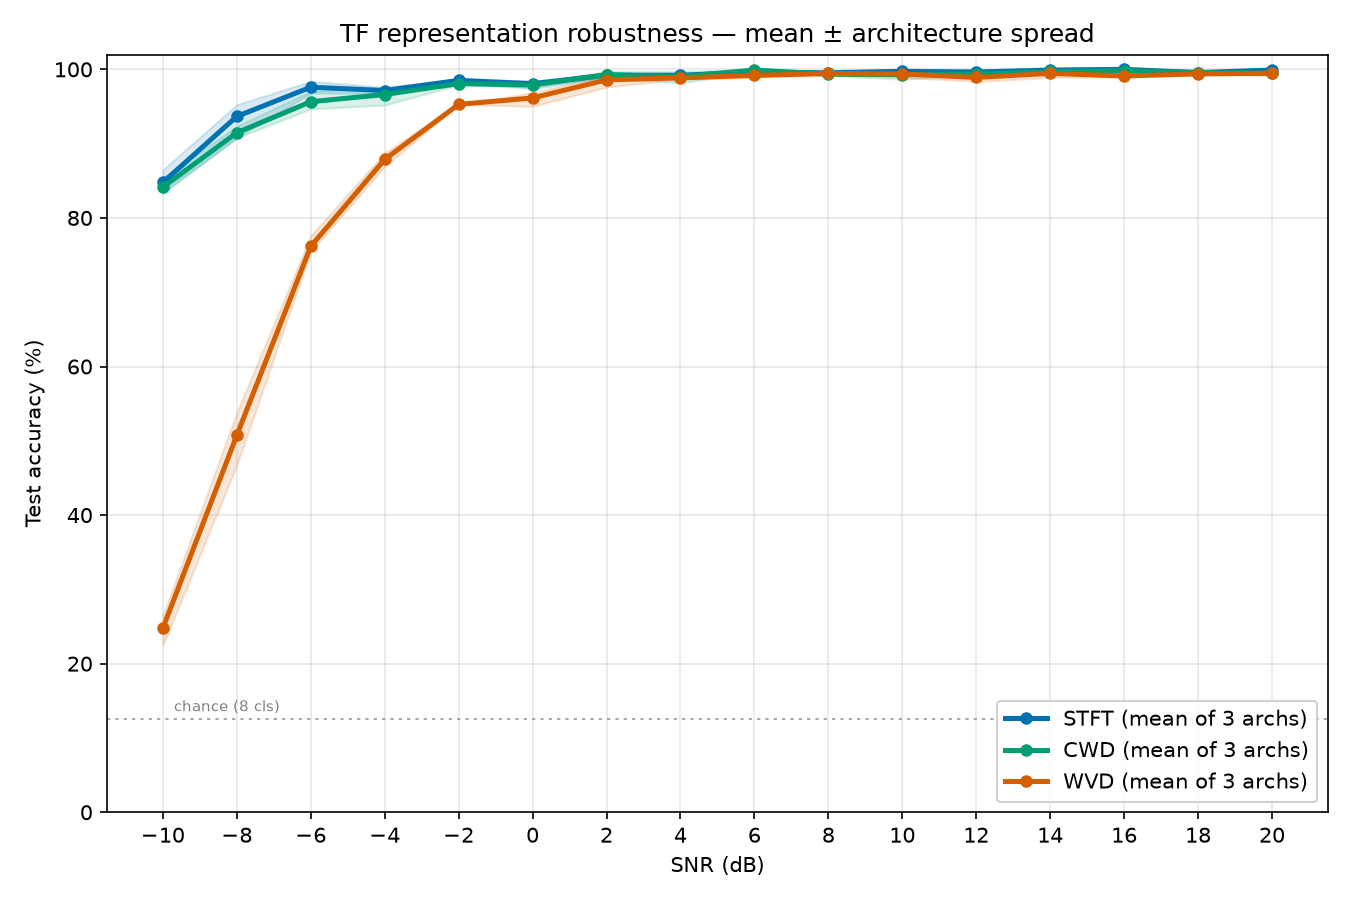
\includegraphics[width=\columnwidth]{tf_family_snr_robustness.png}
\caption{Accuracy vs SNR for the three TF representations (representative seed;
mean over the three architectures, shaded band = min/max across architectures).
The WVD collapses below $-4$~dB while STFT and CWD remain robust.}
\label{fig:robustness}
\end{figure}

\begin{table}[t]
\centering
\caption{Per-SNR accuracy (\%), representation means over architectures for a
representative seed. The STFT$-$WVD gap closes from 60 points at $-10$~dB to under
one point above $+2$~dB.}
\label{tab:lowsnr}
\begin{tabular}{@{}lcccc@{}}
\toprule
SNR & STFT & CWD & WVD & STFT$-$WVD \\
\midrule
$-10$~dB & 84.8 & 84.1 & 24.8 & \textbf{60.0} \\
$-8$~dB  & 93.7 & 91.5 & 50.7 & 42.9 \\
$-6$~dB  & 97.6 & 95.6 & 76.2 & 21.4 \\
$-4$~dB  & 97.1 & 96.6 & 87.9 & 9.3 \\
$-2$~dB  & 98.5 & 98.1 & 95.3 & 3.2 \\
$0$~dB   & 98.1 & 97.9 & 96.2 & 1.9 \\
$\geq\!+6$~dB & 99.7 & 99.6 & 99.3 & $<$1 \\
\bottomrule
\end{tabular}
\end{table}

\subsection{Per-Class Accuracy}
Table~\ref{tab:perclass} breaks the custom-CNN result down by class. Under STFT and
CWD every class exceeds $95\%$ F$_1$; the hardest are the chirp-like LFM and NLFM
and the discrete stepped-frequency waveform, which the confusion analysis
(Fig.~\ref{fig:confusion}) shows are mutually confusable, while the phase-coded
Frank/polyphase codes and the single-tone CW are essentially solved ($\geq99\%$).
The WVD lowers every class by roughly $5$--$11$ points, most on NLFM and SteppedFH,
i.e.\ a broad degradation consistent with its low-SNR collapse rather than a
class-specific failure.

\begin{table}[t]
\centering
\caption{Per-class F$_1$ (\%) for the custom CNN (representative seed).}
\label{tab:perclass}
\begin{tabular}{@{}lccc@{}}
\toprule
Class & STFT & CWD & WVD \\
\midrule
LFM       & 96.8 & 95.9 & 88.5 \\
NLFM      & 96.7 & 96.8 & 85.6 \\
Barker    & 98.3 & 97.6 & 90.5 \\
Frank     & 99.4 & 99.1 & 93.0 \\
Polyphase & 99.1 & 98.8 & 92.0 \\
Costas    & 98.3 & 97.6 & 88.2 \\
CW        & 99.6 & 99.3 & 93.2 \\
SteppedFH & 97.6 & 95.5 & 85.9 \\
\bottomrule
\end{tabular}
\end{table}

\subsection{Statistical Significance}
We assess significance at two levels. \emph{Test-set sampling:} on a
representative (seed-42) run, an unpaired two-proportion $z$-test at the custom-CNN
level finds STFT $>$ CWD to be small but significant ($+0.65$~pt, $p=0.013$), and
STFT/CWD $\gg$ WVD overwhelmingly ($p<10^{-70}$); the corresponding 95\% Wilson
intervals ($n=6000$) are $98.2\%\,[97.9,98.5]$, $97.6\%\,[97.2,97.9]$, and
$89.6\%\,[88.8,90.3]$ for STFT, CWD, and WVD with the custom CNN. A paired McNemar
test on WVD finds the custom CNN better than ResNet-50 ($p<0.001$) and ViT-Small
($p=0.029$).

\emph{Training variance:} these tests cover only test-set sampling, so we also
repeat every experiment across three seeds (Fig.~\ref{fig:multiseed}). The
ordering survives: the STFT, CWD, and WVD accuracy clusters remain mutually
non-overlapping, and STFT exceeds CWD by $0.81$ points---larger than their
combined standard deviation ($0.60$~pt)---so the representation ranking is not an
artefact of a single training run. The custom CNN remains the best or tied
architecture at every representation and, together with ResNet-50, is far more
seed-stable than ViT-Small, which is both the weakest and, by a wide margin, the
least stable.

\begin{figure}[t]
\centering
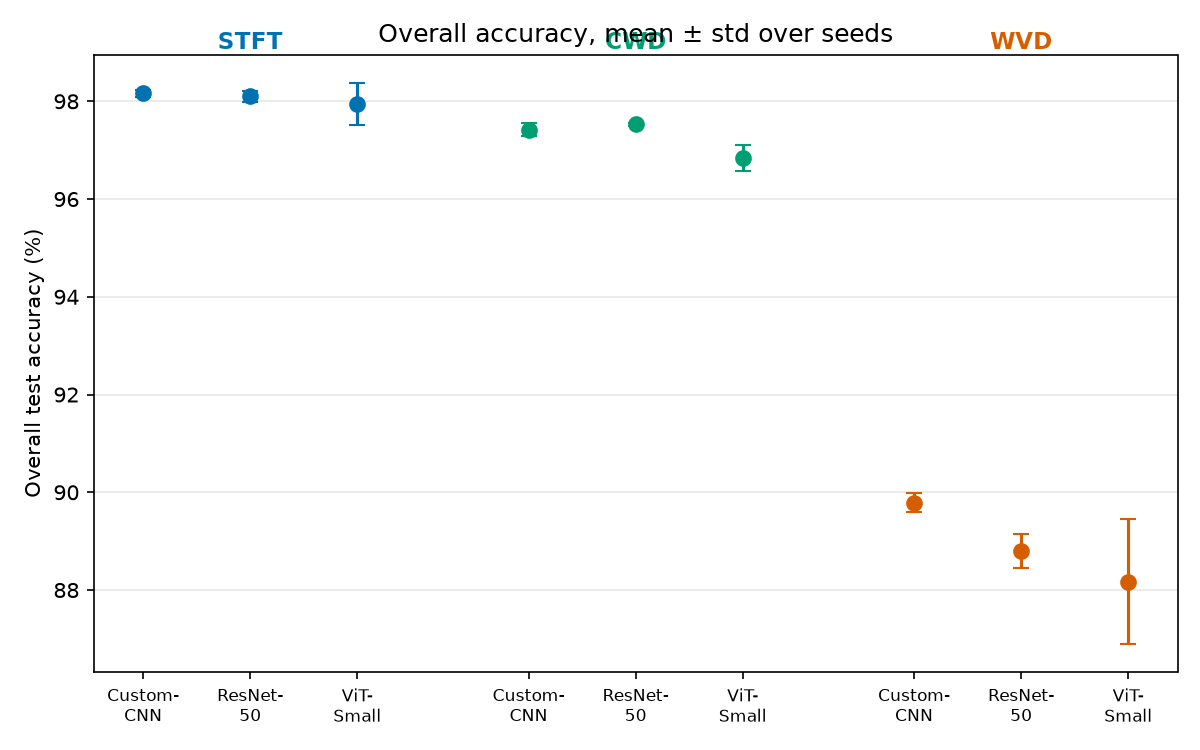
\includegraphics[width=\columnwidth]{multiseed_accuracy.png}
\caption{Overall accuracy per model, mean $\pm$ std over three seeds. The three
representation clusters are mutually non-overlapping; ViT-Small shows the largest
seed variance and the compact CNN the smallest.}
\label{fig:multiseed}
\end{figure}

\subsection{Resource Efficiency}
The smallest model is also the most accurate: the 1.77M-parameter custom CNN
(5.35~GFLOPs) attains the highest mean accuracy overall ($98.16\%$ on STFT), while
ResNet-50 (23.52M, 8.02~GFLOPs) and ViT-Small (21.47M, 8.40~GFLOPs) do not improve
on it. An ImageNet-scale backbone is unnecessary for this eight-class problem.

The representations also differ markedly in computational cost. With on-the-fly
transform computation in the data loader, one training epoch (custom CNN, on our
RTX~5050 laptop GPU) takes about $250$~s for the STFT, $420$~s for the WVD, and
$790$~s for the CWD---the quadratic distributions being $1.7$--$3.2\times$ costlier
than the linear STFT. The STFT is therefore both the most accurate representation
and the cheapest to compute, which together with the compact CNN makes
STFT\,$+$\,custom-CNN the most practical configuration by a clear margin.

%==============================================================================
\section{Discussion}
%==============================================================================
\subsection{Why the WVD Collapses at Low SNR}
The WVD is a quadratic (bilinear) distribution and therefore generates
cross-terms by construction. Although each signal is mono-component, the added
AWGN produces noise$\times$signal and noise$\times$noise cross-terms whose energy
spreads across the entire TF plane; at low SNR these dominate and bury the
authentic signature. The STFT is linear and produces no cross-terms, and the CWD
kernel actively suppresses them, so both degrade gracefully. Above $+2$~dB the
noise cross-terms become negligible and all three converge.

Fig.~\ref{fig:qualitative} makes the mechanism visible: at $+20$~dB the WVD
signature is the sharpest of the three, but by $-10$~dB it is a plane-filling
cross-term speckle, whereas the STFT ridge and CWD signature remain legible.

\begin{figure}[t]
\centering
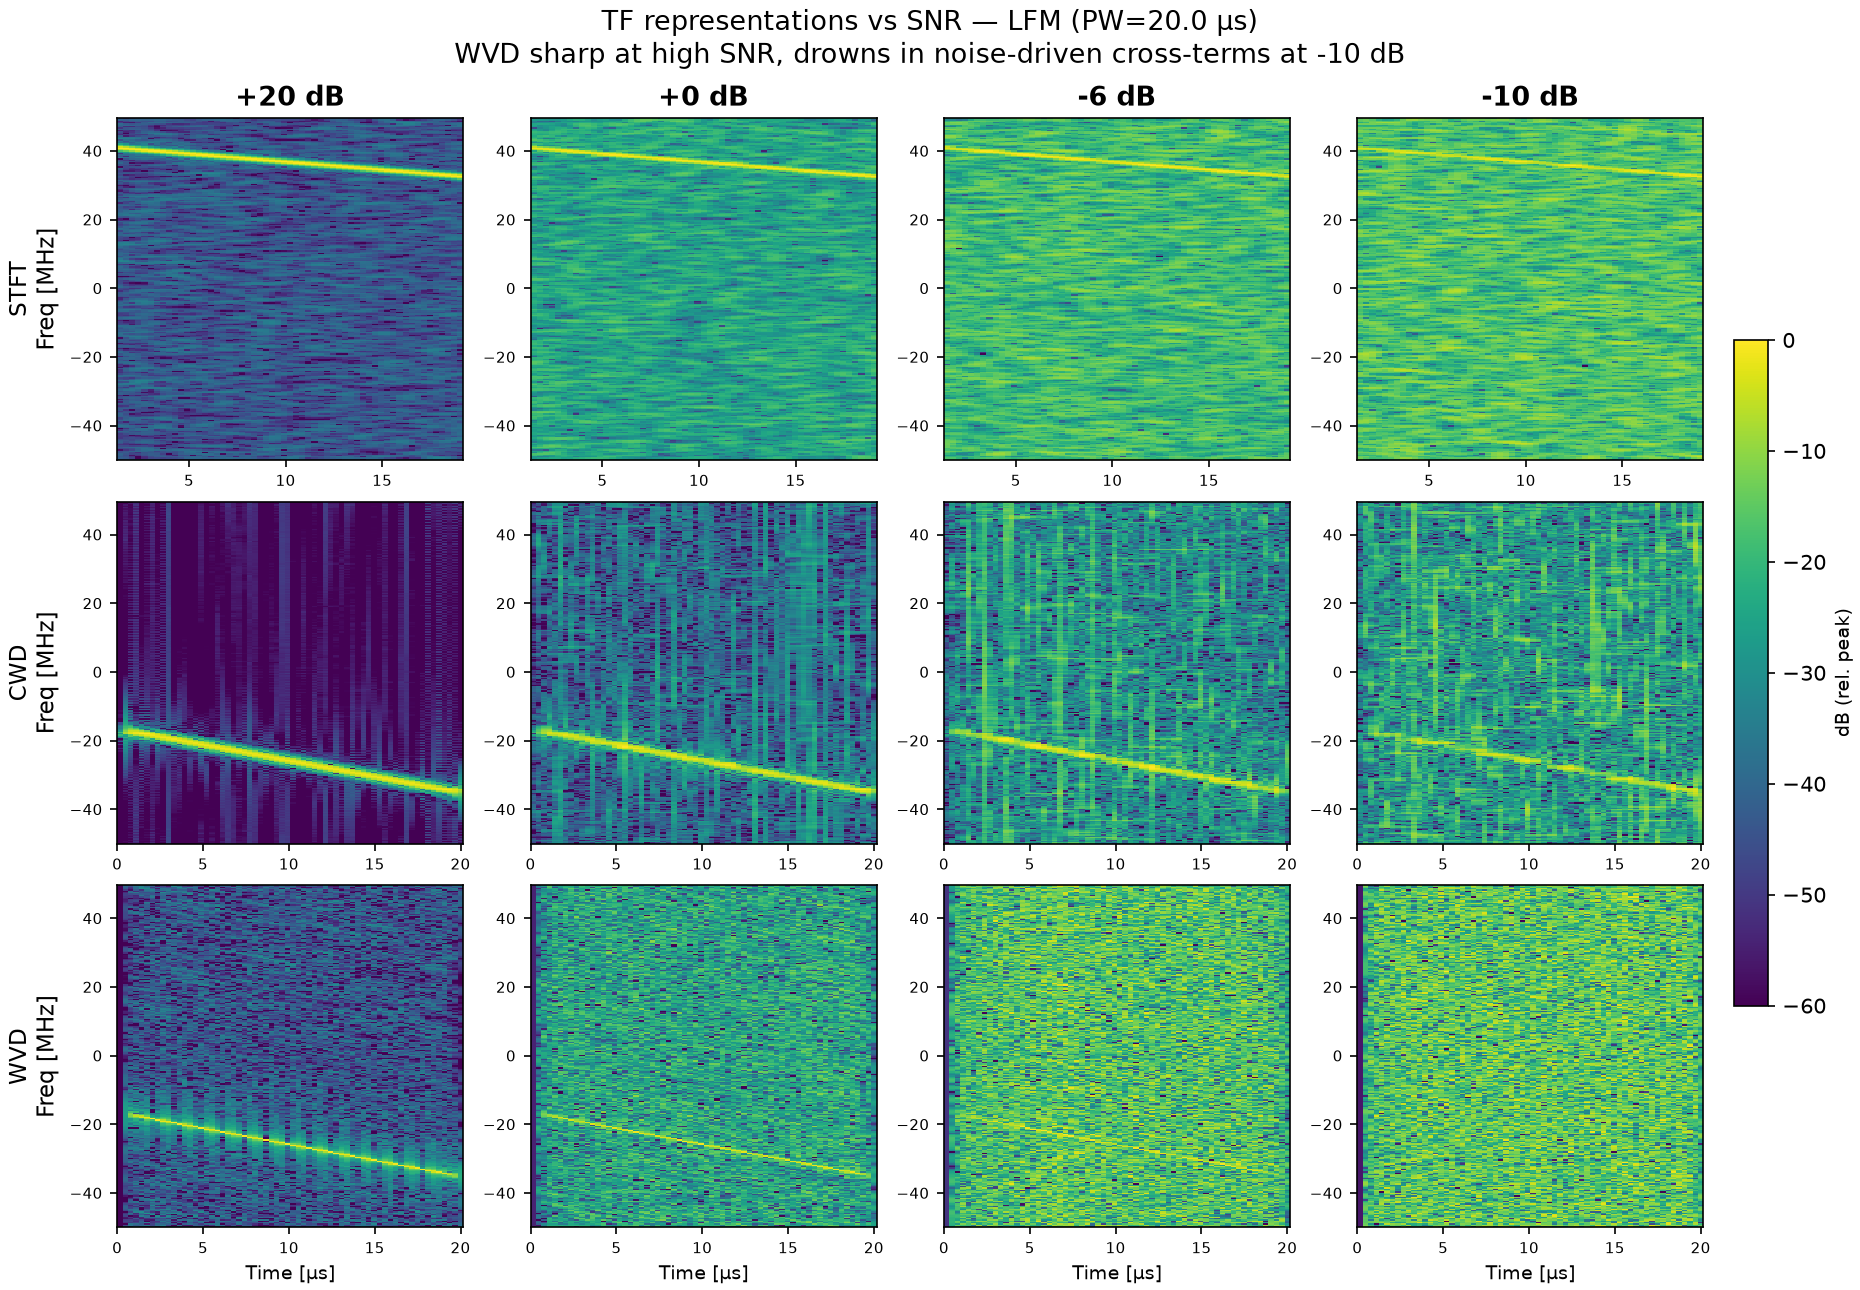
\includegraphics[width=\columnwidth]{qualitative_tf_lfm.png}
\caption{The same LFM pulse under STFT/CWD/WVD (rows) as SNR drops
(columns, $+20/0/-6/-10$~dB). The WVD signature drowns in noise-driven
cross-terms at low SNR while STFT/CWD stay legible.}
\label{fig:qualitative}
\end{figure}

\subsection{What the Model Confuses}
A per-SNR confusion analysis of the WVD models shows the errors change character
with SNR (Fig.~\ref{fig:confusion}): at $-10$~dB the confusion is diffuse, with
predictions smeared toward frequency-agile ``sink'' classes (Costas, SteppedFH,
NLFM)---consistent with a noise-filled plane---whereas by $-6$~dB the errors
concentrate on genuinely similar pairs (LFM$\leftrightarrow$NLFM,
Frank$\leftrightarrow$Polyphase) and the matrix is nearly diagonal.

\begin{figure*}[t]
\centering
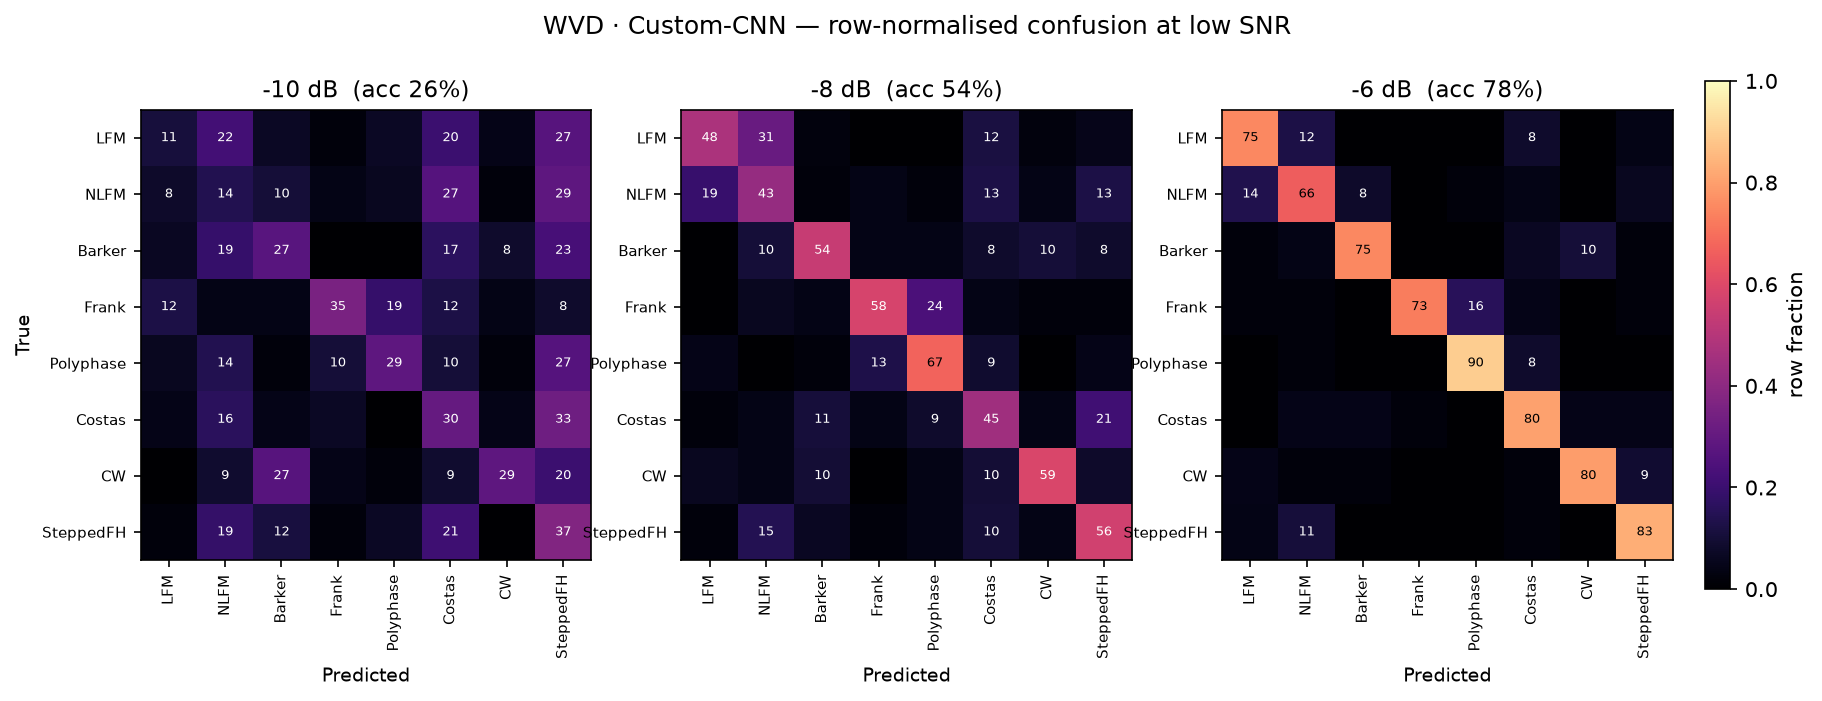
\includegraphics[width=\textwidth]{wvd_lowsnr_confusion_custom_cnn.png}
\caption{Row-normalised confusion for WVD (custom CNN) at $-10$, $-8$, and
$-6$~dB. The errors transition from diffuse and noise-driven at $-10$~dB (mass
scattered toward the frequency-agile classes) to structured intra-family
confusion by $-6$~dB, where the matrix is nearly diagonal.}
\label{fig:confusion}
\end{figure*}

\subsection{Limitations}
Several factors bound the scope of these conclusions. The dataset is synthetic and
mono-component, whereas real intercepts include propagation effects, hardware
impairments, and multiple overlapping emitters; in particular, the WVD's inherent
(signal-on-signal) cross-terms---distinct from the noise-driven cross-terms studied
here---would appear for genuinely multi-component observations. The noise model is
additive white Gaussian applied per pulse (a single look), without clutter,
co-channel interference, or non-Gaussian effects, and without pulse-train
integration that an operational receiver might exploit. The CWD kernel width and
all TF grid sizes are fixed at sensible defaults rather than tuned, so the reported
gaps reflect standard, untuned representations. Finally, our significance analysis
accounts for test-set sampling while the multi-seed study (Table~\ref{tab:main})
bounds training-time variance; the fine-grained ordering among the strong
configurations should be read in that light.

%==============================================================================
\section{Conclusion}
%==============================================================================
On a controlled 3$\times$3 benchmark spanning $-10$ to $+20$~dB, the choice of
time--frequency representation dominates radar pulse classification far more than
the choice of architecture. STFT and CWD are robust across the operational SNR
range, whereas the raw WVD collapses at low SNR---by 60 points at $-10$~dB---owing
to noise-driven cross-term interference. A compact 1.77M-parameter CNN matches
ImageNet-scale backbones, indicating that representation quality, not model
capacity, is the lever for this task. Future work will test these findings on
measured intercepts and multi-component scenarios, and explore adaptive or learned
TF kernels and multi-representation fusion that could combine the WVD's resolution
with the noise robustness of STFT and CWD.

%==============================================================================
\section*{Reproducibility}
%==============================================================================
The data-generation pipeline, training code, frozen split, per-sample test
predictions, and the scripts that regenerate every figure and table are available
at the repository linked on the first page.

\bibliographystyle{IEEEtran}
\bibliography{refs}

\end{document}
